%\nonstopmode
\documentclass[aspectratio=169]{beamer}
\usepackage[utf8]{inputenc}
% \usepackage[frenchb]{babel}
\usepackage{amsmath}
\usepackage{mathtools}
\usepackage{breqn}
\usepackage{multirow}
\usetheme{boxes}
\usepackage{graphicx}
\usepackage{import}
\usepackage{adjustbox}
%\useoutertheme[footline=authortitle,subsection=false]{miniframes}
%\useoutertheme[footline=authorinstitute,subsection=false]{miniframes}
\useoutertheme{infolines}
\setbeamertemplate{headline}{}

\beamertemplatenavigationsymbolsempty

\definecolor{TitleOrange}{RGB}{255,137,0}
\setbeamercolor{title}{fg=TitleOrange}
\setbeamercolor{frametitle}{fg=TitleOrange}

\definecolor{ListOrange}{RGB}{255,145,5}
\setbeamertemplate{itemize item}{\color{ListOrange}$\blacktriangleright$}

\definecolor{verygrey}{RGB}{70,70,70}
\setbeamercolor{normal text}{fg=verygrey}


\usepackage{tabu}
\usepackage{multicol}
\usepackage{vwcol}
\usepackage{stmaryrd}
\usepackage{graphicx}

\usepackage[normalem]{ulem}

\AtBeginSection[]{
  \begin{frame}
  \vfill
  \centering
  \begin{beamercolorbox}[sep=8pt,center,shadow=true,rounded=true]{title}
    \usebeamerfont{title}\insertsectionhead\par%
  \end{beamercolorbox}
  \vfill
  \end{frame}
}

\title{Garage}
\subtitle{a lightweight and robust geo-distributed data storage system}
\author{Alex Auvolat, Deuxfleurs Association}
\date{Inria, 2023-01-18}

\begin{document}

\begin{frame}
	\centering
	
\includegraphics[width=.3\linewidth]{../../sticker/Garage.pdf}
	\vspace{1em}

	{\large\bf Alex Auvolat, Deuxfleurs Association}
	\vspace{1em}

	\url{https://garagehq.deuxfleurs.fr/}

	Matrix channel: \texttt{\#garage:deuxfleurs.fr}
\end{frame}

\begin{frame}
	\frametitle{Who I am}
	\begin{columns}[t]
		\begin{column}{.2\textwidth}
			\centering
			\adjincludegraphics[width=.4\linewidth, valign=t]{assets/alex.jpg}
		\end{column}
		\begin{column}{.6\textwidth}
			\textbf{Alex Auvolat}\\
			PhD; co-founder of Deuxfleurs
		\end{column}
		\begin{column}{.2\textwidth}
			~
		\end{column}
	\end{columns}
	\vspace{2em}

	\begin{columns}[t]
		\begin{column}{.2\textwidth}
			\centering
			\adjincludegraphics[width=.5\linewidth, valign=t]{assets/deuxfleurs.pdf}
		\end{column}
		\begin{column}{.6\textwidth}
			\textbf{Deuxfleurs}\\
			A non-profit self-hosting collective,\\
			member of the CHATONS network
		\end{column}
		\begin{column}{.2\textwidth}
			\centering
			\adjincludegraphics[width=.7\linewidth, valign=t]{assets/logo_chatons.png}
		\end{column}
	\end{columns}

\end{frame}

\begin{frame}
	\frametitle{Our objective at Deuxfleurs}
	
	\begin{center}
		\textbf{Promote self-hosting and small-scale hosting\\
			as an alternative to large cloud providers}
	\end{center}
	\vspace{2em}
	\visible<2->{
		Why is it hard?
	}
	\visible<3->{
		\vspace{2em}
		\begin{center}
			\textbf{\underline{Resilience}}\\
			{\footnotesize (we want good uptime/availability with low supervision)}
		\end{center}
	}
\end{frame}

\begin{frame}
	\frametitle{How to make a \underline{stable} system}

	Enterprise-grade systems typically employ:
	\vspace{1em}
	\begin{itemize}
		\item RAID
		\item Redundant power grid + UPS
		\item Redundant Internet connections
		\item Low-latency links
		\item ... 
	\end{itemize}
	\vspace{1em}
	$\to$ it's costly and only worth it at DC scale
\end{frame}

\begin{frame}
	\frametitle{How to make a \underline{resilient} system}

	\only<1,4-5>{
		Instead, we use:
		\vspace{1em}
		\begin{itemize}
			\item \textcolor<2->{gray}{Commodity hardware (e.g. old desktop PCs)}
				\vspace{.5em}
			\item<4-> \textcolor<5->{gray}{Commodity Internet (e.g. FTTB, FTTH) and power grid}
				\vspace{.5em}
			\item<5-> \textcolor<6->{gray}{\textbf{Geographical redundancy} (multi-site replication)}
		\end{itemize}
	}
	\only<2>{
		\begin{center}
			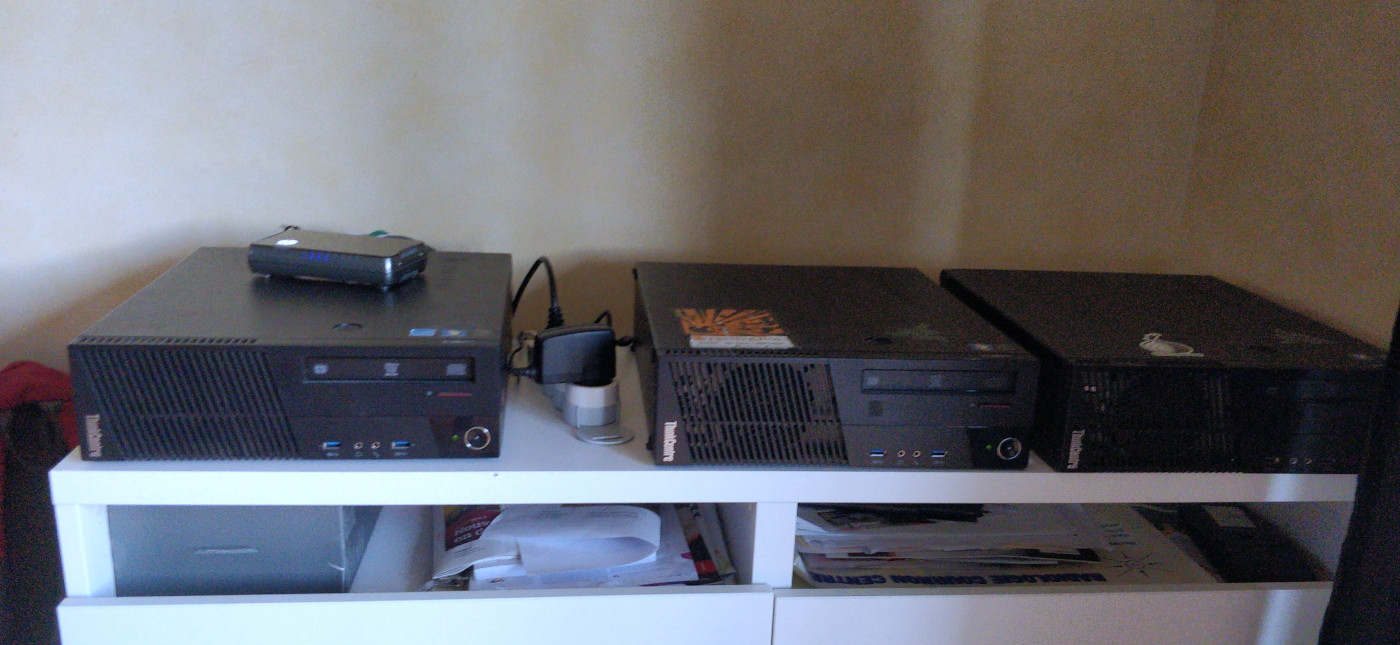
\includegraphics[width=.8\linewidth]{assets/atuin.jpg}
		\end{center}
	}
	\only<3>{
		\begin{center}
			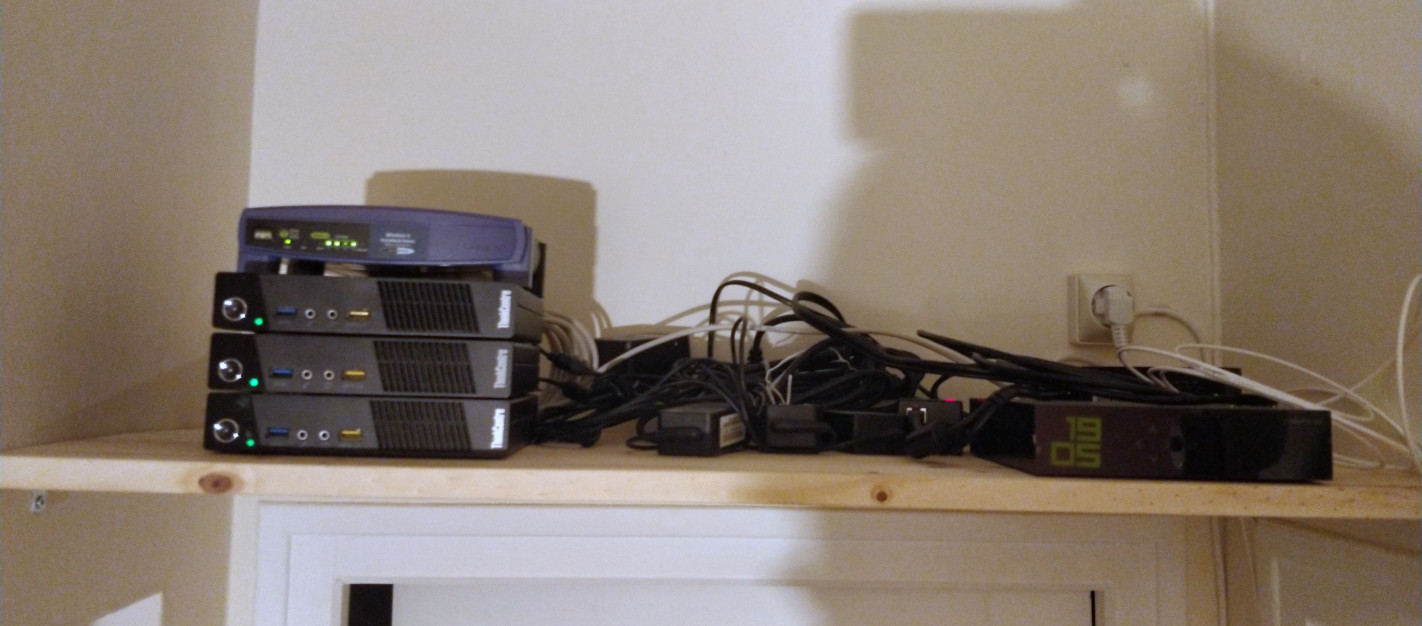
\includegraphics[width=.8\linewidth]{assets/neptune.jpg}
		\end{center}
	}
	\only<6>{
		\begin{center}
			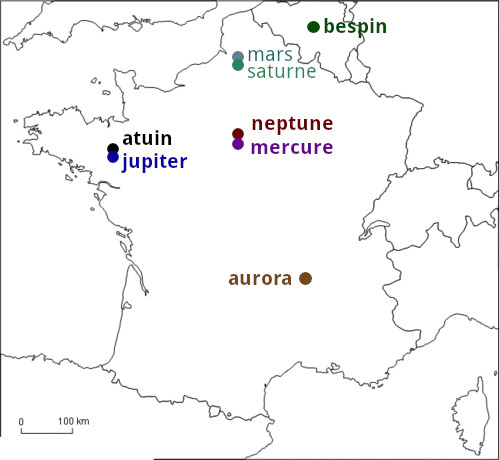
\includegraphics[width=.5\linewidth]{assets/inframap.jpg}
		\end{center}
	}
\end{frame}

\begin{frame}
	\frametitle{How to make this happen}
	\begin{center}
		\only<1>{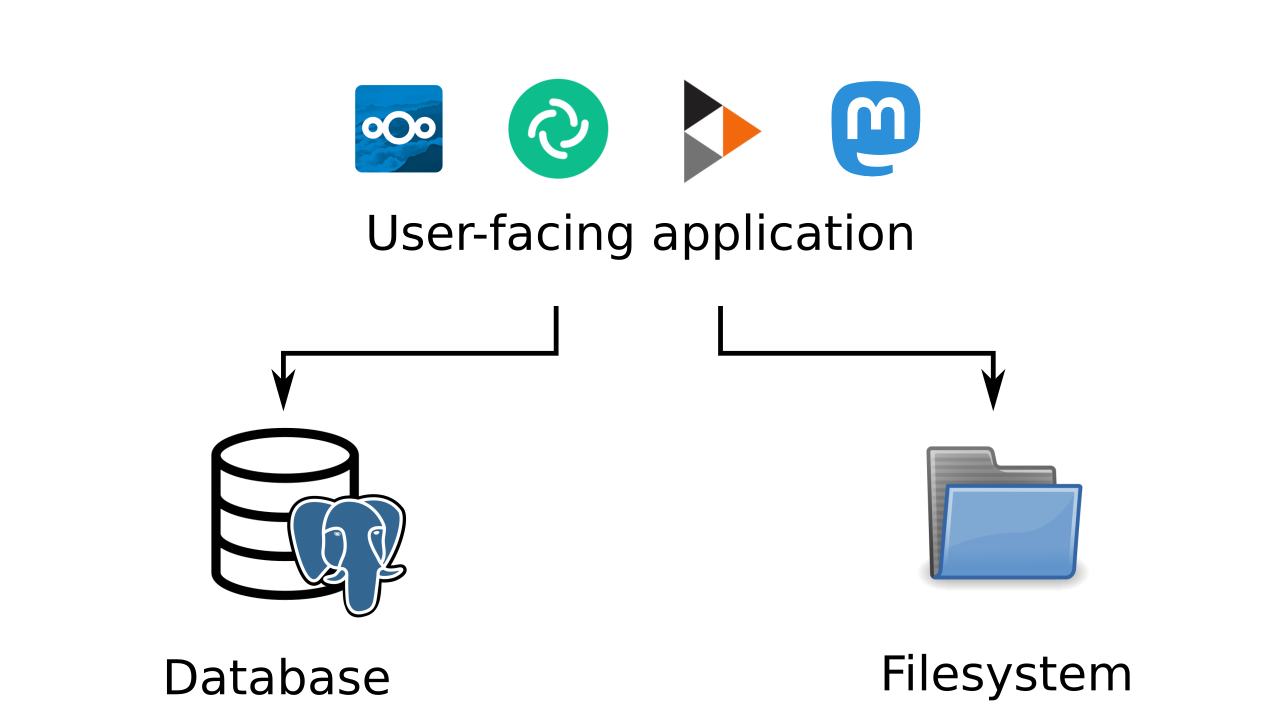
\includegraphics[width=.8\linewidth]{assets/slide1.png}}%
		\only<2>{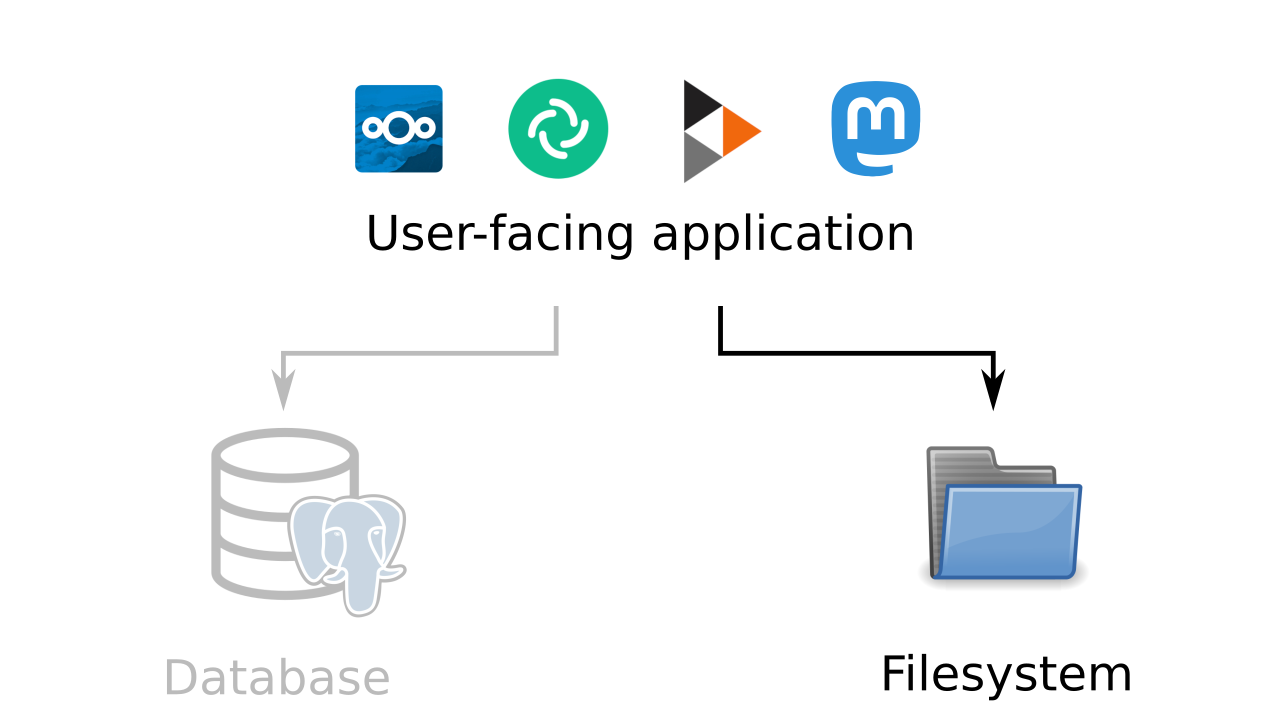
\includegraphics[width=.8\linewidth]{assets/slide2.png}}%
		\only<3>{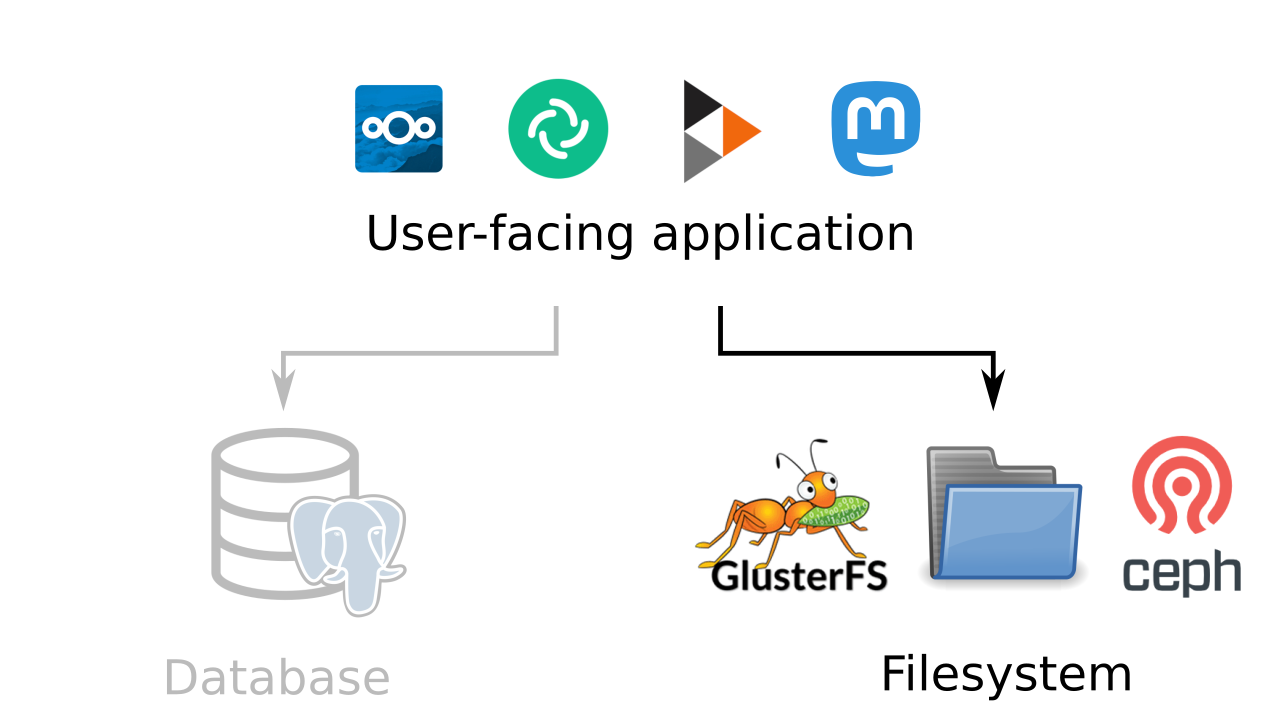
\includegraphics[width=.8\linewidth]{assets/slide3.png}}%
	\end{center}
\end{frame}

\begin{frame}
	\frametitle{Distributed file systems are slow}
	File systems are complex, for example:
	\vspace{1em}
	\begin{itemize}
		\item Concurrent modification by several processes
			\vspace{1em}
		\item Folder hierarchies
			\vspace{1em}
		\item Other requirements of the POSIX spec
	\end{itemize}
	\vspace{1em}
	Coordination in a distributed system is costly

	\vspace{1em}
	Costs explode with commodity hardware / Internet connections\\
	{\small (we experienced this!)}
\end{frame}

\begin{frame}
	\frametitle{A simpler solution: object storage}
	Only two operations:
	\vspace{1em}
	\begin{itemize}
		\item Put an object at a key
			\vspace{1em}
		\item Retrieve an object from its key
	\end{itemize}
	\vspace{1em}
	{\footnotesize (and a few others)}

	\vspace{1em}
	Sufficient for many applications!
\end{frame}

\begin{frame}
	\frametitle{A simpler solution: object storage}
		\begin{center}
			
\includegraphics[height=6em]{../2020-12-02_wide-team/img/Amazon-S3.jpg}
			\hspace{3em}
			
\includegraphics[height=5em]{assets/minio.png}
			\hspace{3em}
			
\includegraphics[height=6em]{../../logo/garage_hires_crop.png}
		\end{center}
		\vspace{1em}
	S3: a de-facto standard, many compatible applications

	\vspace{1em}

	MinIO is self-hostable but not suited for geo-distributed deployments

	\vspace{1em}

	\textbf{Garage is a self-hosted drop-in replacement for the Amazon S3 object store}
\end{frame}


\begin{frame}
	\frametitle{The data model of object storage}
	Object storage is basically a key-value store:
	\vspace{1em}

		\begin{center}
		\begin{tabular}{|l|p{8cm}|}
			\hline
			\textbf{Key: file path + name} & \textbf{Value: file data + metadata} \\
			\hline
			\hline
			\texttt{index.html} &
				\texttt{Content-Type: text/html; charset=utf-8} \newline
				\texttt{Content-Length: 24929} \newline
				\texttt{<binary blob>} \\ 
			\hline
			\texttt{img/logo.svg} &
				\texttt{Content-Type: text/svg+xml} \newline
				\texttt{Content-Length: 13429} \newline
				\texttt{<binary blob>} \\ 
			\hline
			\texttt{download/index.html} &
				\texttt{Content-Type: text/html; charset=utf-8} \newline
				\texttt{Content-Length: 26563} \newline
				\texttt{<binary blob>} \\ 
			\hline
		\end{tabular}
		\end{center}

\end{frame}

\begin{frame}
	\frametitle{Two big problems}
	\begin{enumerate}
		\item \textbf{How to place data on different nodes?}\\
			\vspace{1em}
			\underline{Constraints:} heterogeneous hardware\\
			\underline{Objective:} $n$ copies of everything, maximize usable capacity, maximize resilience\\
			\vspace{1em}
			$\to$ the Dynamo model + optimization algorithms
			\vspace{2em}
		\item<2-> \textbf{How to guarantee consistency?}\\
			\vspace{1em}
			\underline{Constraints:} slow network (geographical distance), node unavailability/crashes\\
			\underline{Objective:} maximize availability, read-after-write guarantee\\
			\vspace{1em}
			$\to$ CRDTs, monotonicity, read and write quorums
	\end{enumerate}
\end{frame}

\section{Problem 1: placing data}

\begin{frame}
	\frametitle{Key-value stores, upgraded: the Dynamo model}
	\textbf{Two keys:}
	\begin{itemize}
		\item Partition key: used to divide data into partitions (shards)
		\item Sort key: used to identify items inside a partition
	\end{itemize}

	\vspace{1em}

	\begin{center}
	\begin{tabular}{|l|l|p{3cm}|}
		\hline
		\textbf{Partition key: bucket} & \textbf{Sort key: filename} & \textbf{Value} \\
		\hline
		\hline
		\texttt{website} & \texttt{index.html} & (file data) \\
		\hline
		\texttt{website} & \texttt{img/logo.svg} & (file data) \\
		\hline
		\texttt{website} & \texttt{download/index.html} & (file data) \\
		\hline
		\hline
		\texttt{backup} & \texttt{borg/index.2822} & (file data) \\
		\hline
		\texttt{backup} & \texttt{borg/data/2/2329} & (file data) \\
		\hline
		\texttt{backup} & \texttt{borg/data/2/2680} & (file data) \\
		\hline
		\hline
		\texttt{private} & \texttt{qq3a2nbe1qjq0ebbvo6ocsp6co} & (file data) \\
		\hline
	\end{tabular}
	\end{center}
\end{frame}

\begin{frame}
	\frametitle{Key-value stores, upgraded: the Dynamo model}
	\begin{itemize}
		\item Data with different partition keys is stored independantly,\\
			on a different set of nodes\\
			\vspace{.5em}
			$\to$ no easy way to list all partition keys\\
			$\to$ no cross-shard transactions\\
			\vspace{2em}
		\item Placing data: hash the partition key, select nodes accordingly\\
			\vspace{.5em}
			$\to$ distributed hash table (DHT)
			\vspace{2em}
		\item For a given value of the partition key, items can be listed using their sort keys
	\end{itemize}
\end{frame}

\begin{frame}
	\frametitle{How to spread files over different cluster nodes?}
	\textbf{Consistent hashing (Dynamo):}
	\vspace{1em}

	\begin{center}
	\only<1>{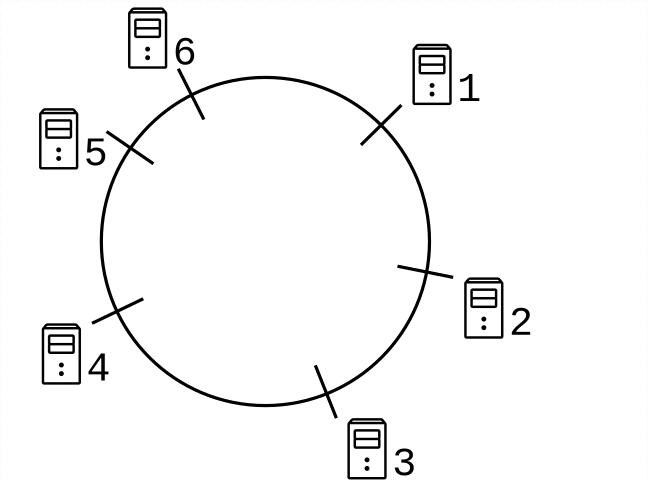
\includegraphics[width=.40\columnwidth]{assets/consistent_hashing_1.pdf}}%
	\only<2>{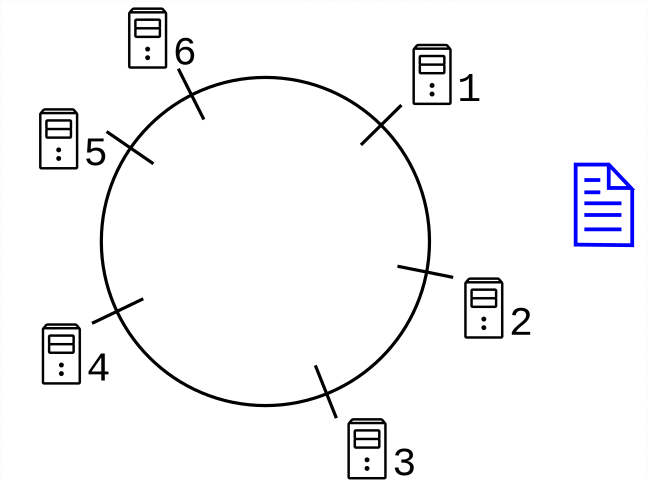
\includegraphics[width=.40\columnwidth]{assets/consistent_hashing_2.pdf}}%
	\only<3>{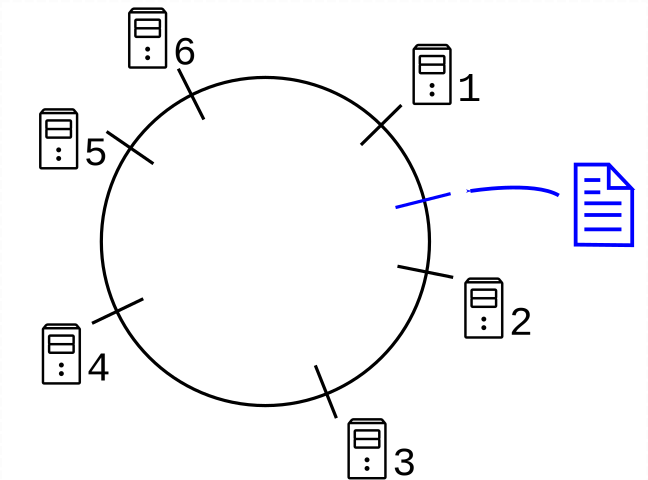
\includegraphics[width=.40\columnwidth]{assets/consistent_hashing_3.pdf}}%
	\only<4>{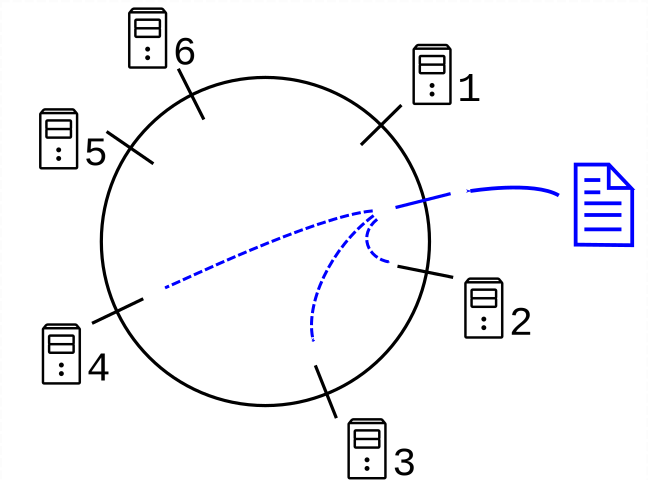
\includegraphics[width=.40\columnwidth]{assets/consistent_hashing_4.pdf}}%
	\end{center}
\end{frame}

\begin{frame}
	\frametitle{Constraint: location-awareness}
	\begin{center}
		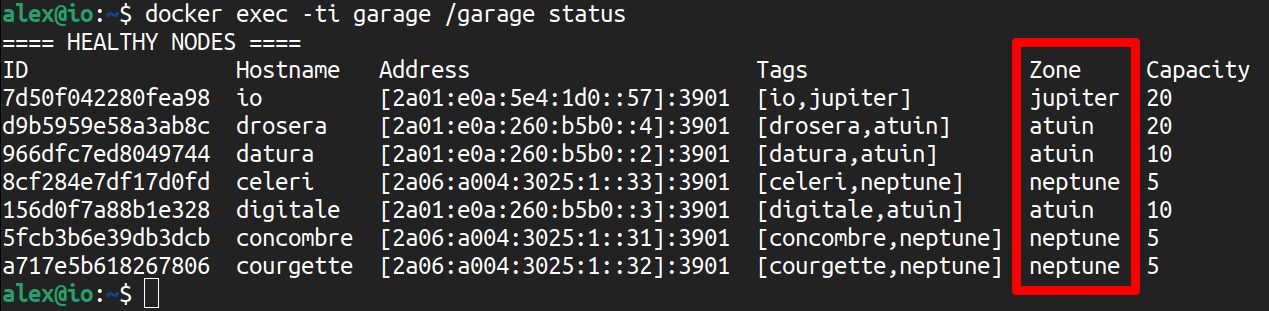
\includegraphics[width=\linewidth]{assets/location-aware.png}
	\end{center}
	\vspace{2em}
	Garage replicates data on different zones when possible
\end{frame}

\begin{frame}
	\frametitle{Constraint: location-awareness}
		\begin{center}
			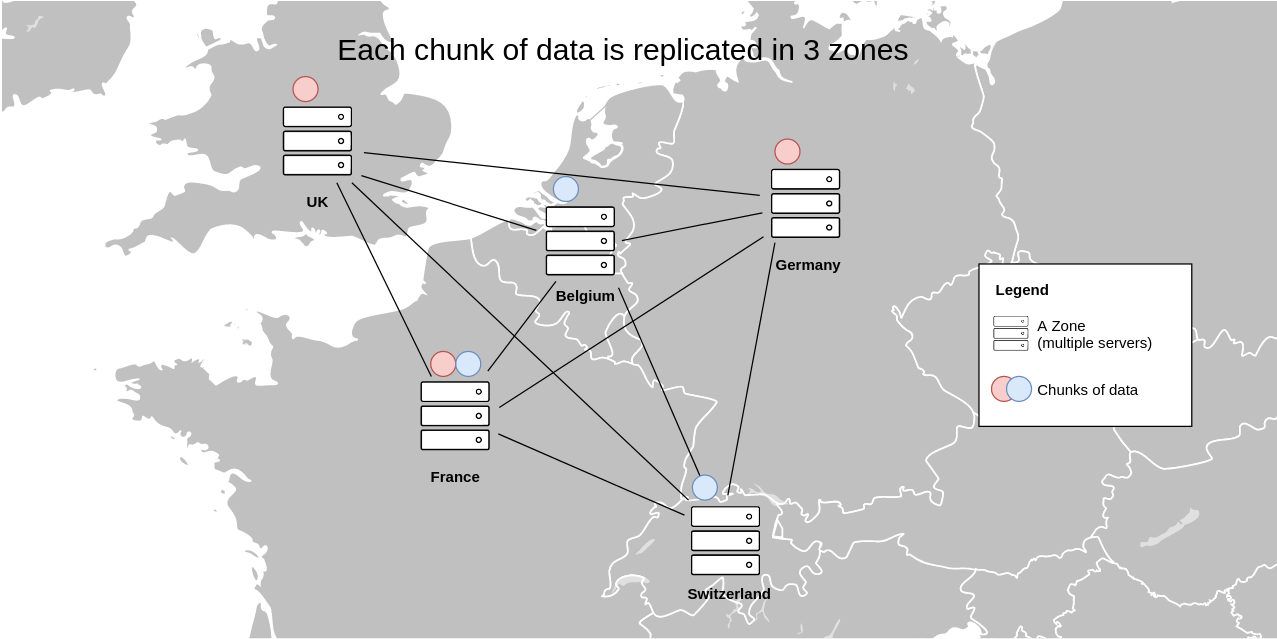
\includegraphics[width=.8\linewidth]{assets/map.png}
		\end{center}
\end{frame}

\begin{frame}
	\frametitle{Issues with consistent hashing}
	\begin{itemize}
		\item Consistent hashing doesn't dispatch data based on geographical location of nodes
			\vspace{1em}
		\item<2-> Geographically aware adaptation, try 1:\\
			data quantities not well balanced between nodes
			\vspace{1em}
		\item<3-> Geographically aware adaptation, try 2:\\
			too many reshuffles when adding/removing nodes
	\end{itemize}
\end{frame}

\begin{frame}
	\frametitle{How to spread files over different cluster nodes?}
	\textbf{Garage's method: build an index table}
	\vspace{1em}

	Realization: we can actually precompute an optimal solution
	\vspace{1em}

	\visible<2->{
		\begin{center}
		\begin{tabular}{|l|l|l|l|}
			\hline
			\textbf{Partition} & \textbf{Node 1} & \textbf{Node 2} & \textbf{Node 3} \\
			\hline
			\hline
			Partition 0 & Io (jupiter) & Drosera (atuin) & Courgette (neptune) \\
			\hline
			Partition 1 & Datura (atuin) & Courgette (neptune) & Io (jupiter) \\
			\hline
			Partition 2 & Io(jupiter) & Celeri (neptune) & Drosera (atuin) \\
			\hline
			\hspace{1em}$\vdots$ & \hspace{1em}$\vdots$ & \hspace{1em}$\vdots$ & \hspace{1em}$\vdots$ \\
			\hline
			Partition 255 & Concombre (neptune) & Io (jupiter) & Drosera (atuin) \\
			\hline
		\end{tabular}
		\end{center}
	}
	\vspace{1em}
	\visible<3->{
		The index table is built centrally using an optimal algorithm,\\
		then propagated to all nodes
	}
\end{frame}

\begin{frame}
	\frametitle{The relationship between \emph{partition} and \emph{partition key}}
	\begin{center}
	\begin{tabular}{|l|l|l|l|}
		\hline
		\textbf{Partition key} & \textbf{Partition} & \textbf{Sort key} & \textbf{Value} \\
		\hline
		\hline
		\texttt{website} & Partition 12 & \texttt{index.html} & (file data) \\
		\hline
		\texttt{website} & Partition 12 & \texttt{img/logo.svg} & (file data) \\
		\hline
		\texttt{website} & Partition 12 &\texttt{download/index.html} & (file data) \\
		\hline
		\hline
		\texttt{backup} & Partition 42 & \texttt{borg/index.2822} & (file data) \\
		\hline
		\texttt{backup} & Partition 42 & \texttt{borg/data/2/2329} & (file data) \\
		\hline
		\texttt{backup} & Partition 42 & \texttt{borg/data/2/2680} & (file data) \\
		\hline
		\hline
		\texttt{private} & Partition 42 & \texttt{qq3a2nbe1qjq0ebbvo6ocsp6co} & (file data) \\
		\hline
	\end{tabular}
	\end{center}
	\vspace{1em}
	\textbf{To read or write an item:} hash partition key
	\\ \hspace{5cm} $\to$ determine partition number (first 8 bits)
	\\ \hspace{5cm} $\to$ find associated nodes
\end{frame}

\begin{frame}
	\frametitle{Garage's internal data structures}
	\centering
	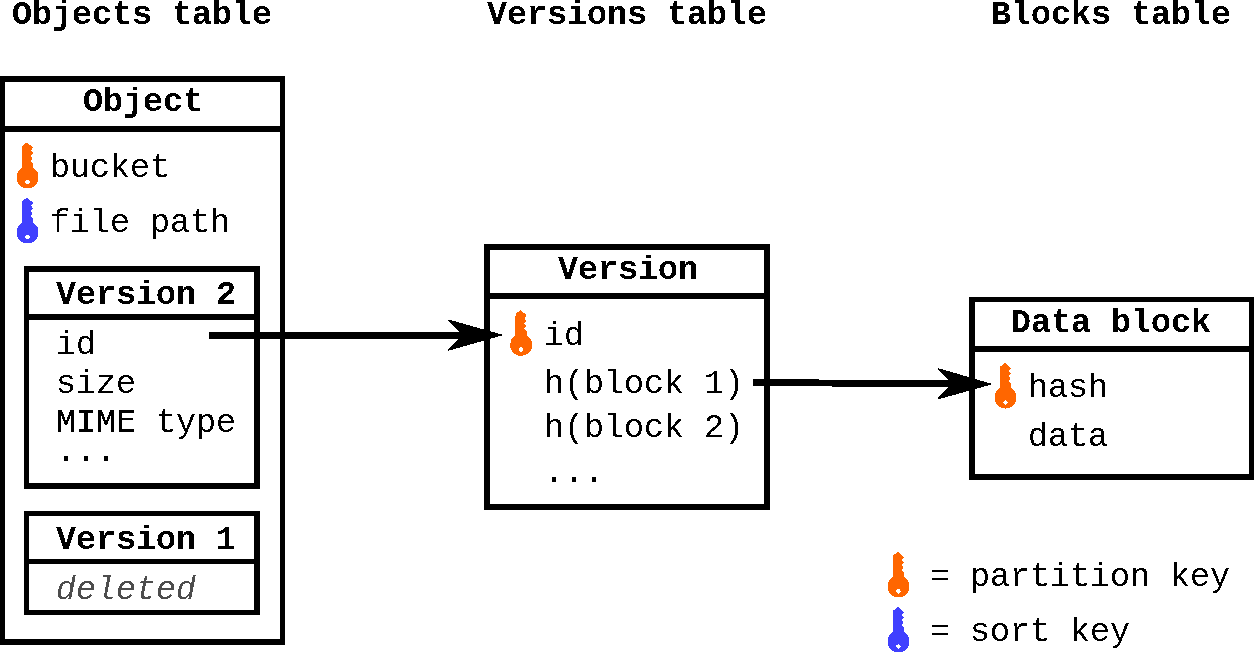
\includegraphics[width=.75\columnwidth]{assets/garage_tables.pdf}
\end{frame}

\begin{frame}
	\frametitle{Storing and retrieving files}
	\begin{center}
		\only<1>{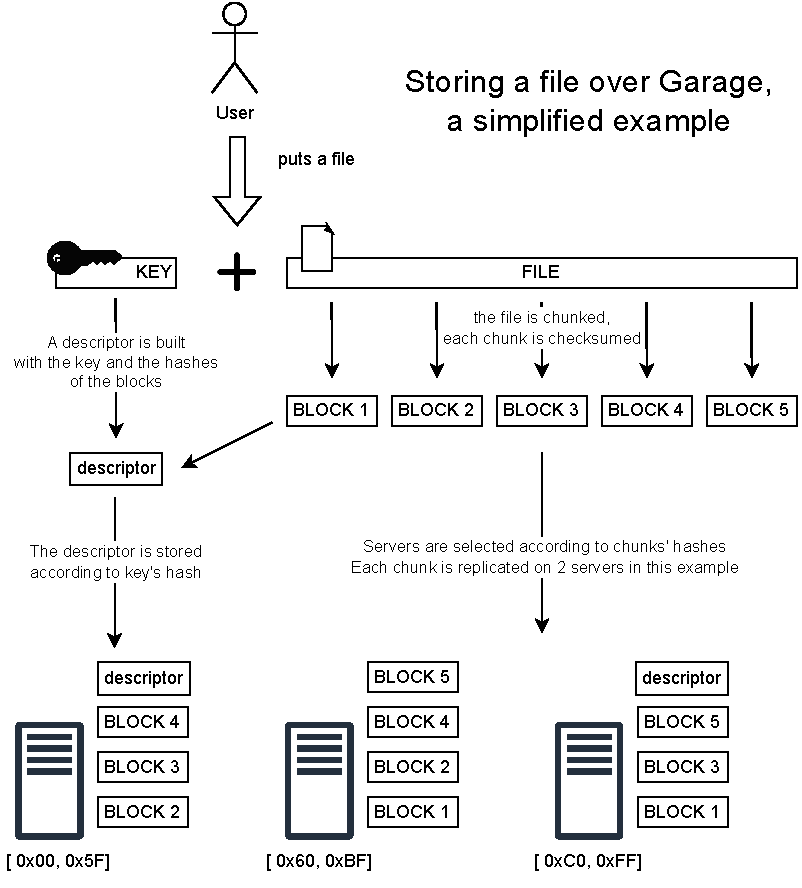
\includegraphics[width=.45\linewidth]{assets/garage2a.drawio.pdf}}%
		\only<2>{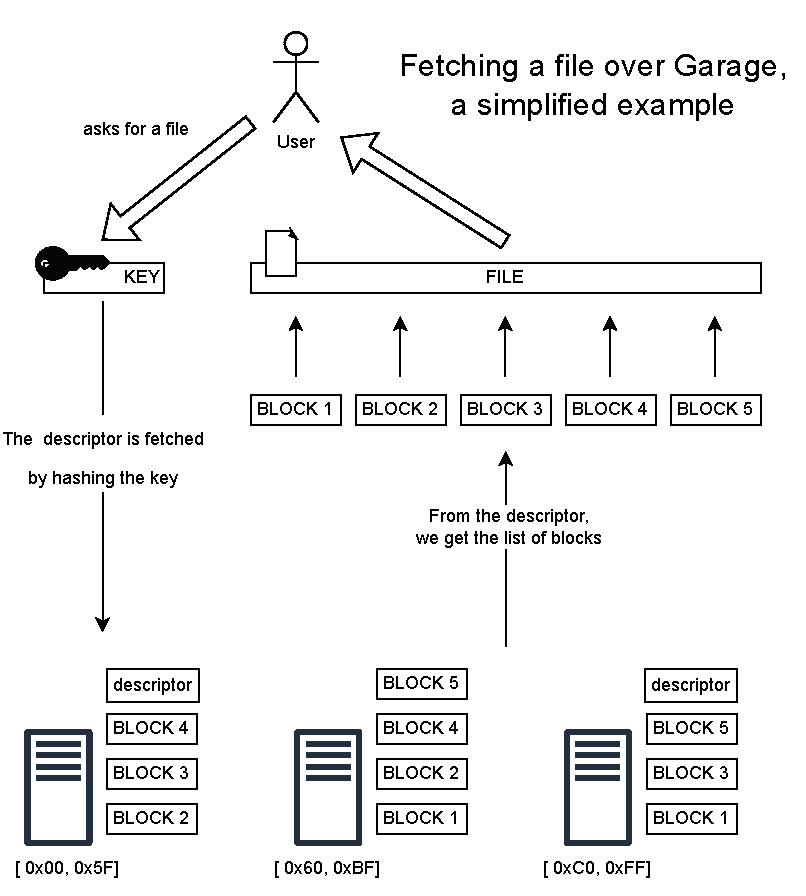
\includegraphics[width=.45\linewidth]{assets/garage2b.drawio.pdf}}%
	\end{center}
\end{frame}

\section{Problem 2: ensuring consistency}

\begin{frame}
	\frametitle{Consensus vs weak consistency}

	\hspace{1em}
	\begin{minipage}{7cm}
		\textbf{Consensus-based systems:}
		\vspace{1em}
		\begin{itemize}
			\item \textbf{Leader-based:} a leader is elected to coordinate
				all reads and writes
				\vspace{1em}
			\item \textbf{Linearizability} of all operations\\
				(strongest consistency guarantee)
				\vspace{1em}
			\item Any sequential specification can be implemented as a \textbf{replicated state machine}
				\vspace{1em}
			\item \textbf{Costly}, the leader is a bottleneck;
				leader elections on failure take time
		\end{itemize}
	\end{minipage}
	\hfill
	\begin{minipage}{7cm} \visible<2->{
		\textbf{Weakly consistent systems:}
		\vspace{1em}
		\begin{itemize}
			\item \textbf{Nodes are equivalent}, any node
				can originate a read or write operation
				\vspace{1em}
			\item \textbf{Read-after-write consistency} with quorums,
				eventual consistency without
				\vspace{1em}
			\item \textbf{Operations have to commute}, i.e.~we
				can only implement CRDTs
				\vspace{1em}
			\item \textbf{Fast}, no single bottleneck;\\
				works the same with offline nodes
		\end{itemize}
	} \end{minipage}
	\hspace{1em}
\end{frame}

\begin{frame}
	\frametitle{Consensus vs weak consistency}
	\begin{center}
		\textbf{The same objects cannot be implemented in both models.}
	\end{center}
	\vspace{2em}

	\hspace{1em}
	\begin{minipage}{6.5cm}
		\underline{Consensus-based systems:}

		\vspace{1em}

		\textbf{Any sequential specification}\\~

		\vspace{1em}
		\textbf{Easier to program for}: just write your program as if it were sequential on a single machine

	\end{minipage}
	\hfill
	\begin{minipage}{6.5cm}
		\underline{Weakly consistent systems:}

		\vspace{1em}
		
		\textbf{Limited objects such as CRDTs}\\(conflict-free replicated data types)

		\vspace{1em}
		Part of the complexity is \textbf{reported to the consumer of the API}\\~
	\end{minipage}
	\hspace{1em}
\end{frame}

\begin{frame}
	\frametitle{Consensus vs weak consistency}
	\begin{center}
		\textbf{From a theoretical point of view:}\\

	\end{center}
	\vspace{2em}

	\hspace{1em}
	\begin{minipage}{6.5cm}
		\underline{Consensus-based systems:}

		\vspace{1em}

		Require \textbf{additionnal assumptions} such as a fault detector or a strong RNG\\~
	\end{minipage}
	\hfill
	\begin{minipage}{6.5cm}
		\underline{Weakly consistent systems:}

		\vspace{1em}
		
		Can be implemented in \textbf{any asynchronous message passing distributed system}
	\end{minipage}
	\hspace{1em}

	\vspace{3em}
	\begin{center}
		They represent \textbf{different classes of computational capability}
	\end{center}
\end{frame}

\begin{frame}
	\frametitle{Understanding the power of consensus}
	\textbf{Consensus:} an API with a single operation, $propose(x)$
	\begin{enumerate}
		\item nodes all call $propose(x)$ with their proposed value;
		\item nodes all receive the same value as a return value, which is one of the proposed values
	\end{enumerate}
	\vspace{1em}
	
	\visible<2->{
		\textbf{Equivalent to} a distributed algorithm that gives a total order on all requests
	}
	\vspace{1em}

	\visible<3->{
		\textbf{Implemented by} this simple replicated state machine:
		\vspace{.5em}
		\begin{figure}
			\centering
			\def\svgwidth{.5\textwidth}
			\large
			\import{assets/}{consensus.pdf_tex}
		\end{figure}
		\vspace{1em}
	}
\end{frame}

\begin{frame}
	\frametitle{Can my object be implemented without consensus?}
	\underline{Given the specification of an API:}
	\vspace{2em}
	\begin{itemize}
		\item \textbf{Using this API, we can implement the consensus object} (the $propose$ function)\\
			$\to$ the API is equivalent to consensus/total ordering of messages\\
			$\to$ the API cannot be implemented in a weakly consistent system
			\vspace{2em}
		\item \textbf{This API can be implemented using only weak primitives}\\
			(e.g. a bunch of atomic registers)\\
			$\to$ the API is strictly weaker than consensus\\
			$\to$ we can implement it in Garage!
	\end{itemize}
\end{frame}

\begin{frame}
	\frametitle{Why avoid consensus?}
	Consensus can be implemented reasonably well in practice, so why avoid it?
	\vspace{2em}
	\begin{itemize}
		\item \textbf{Software complexity:} RAFT and PAXOS are complex beasts;\\
			harder to prove, harder to reason about
			\vspace{1.5em}
		\item \textbf{Performance issues:}
			\vspace{1em}
			\begin{itemize}
				\item The leader is a \textbf{bottleneck} for all requests
					\vspace{1em}
				\item Particularly \textbf{sensitive to higher latency} between nodes
			\end{itemize}
	\end{itemize}
\end{frame}

\begin{frame}
	\frametitle{Performance gains in practice}
	\begin{center}
		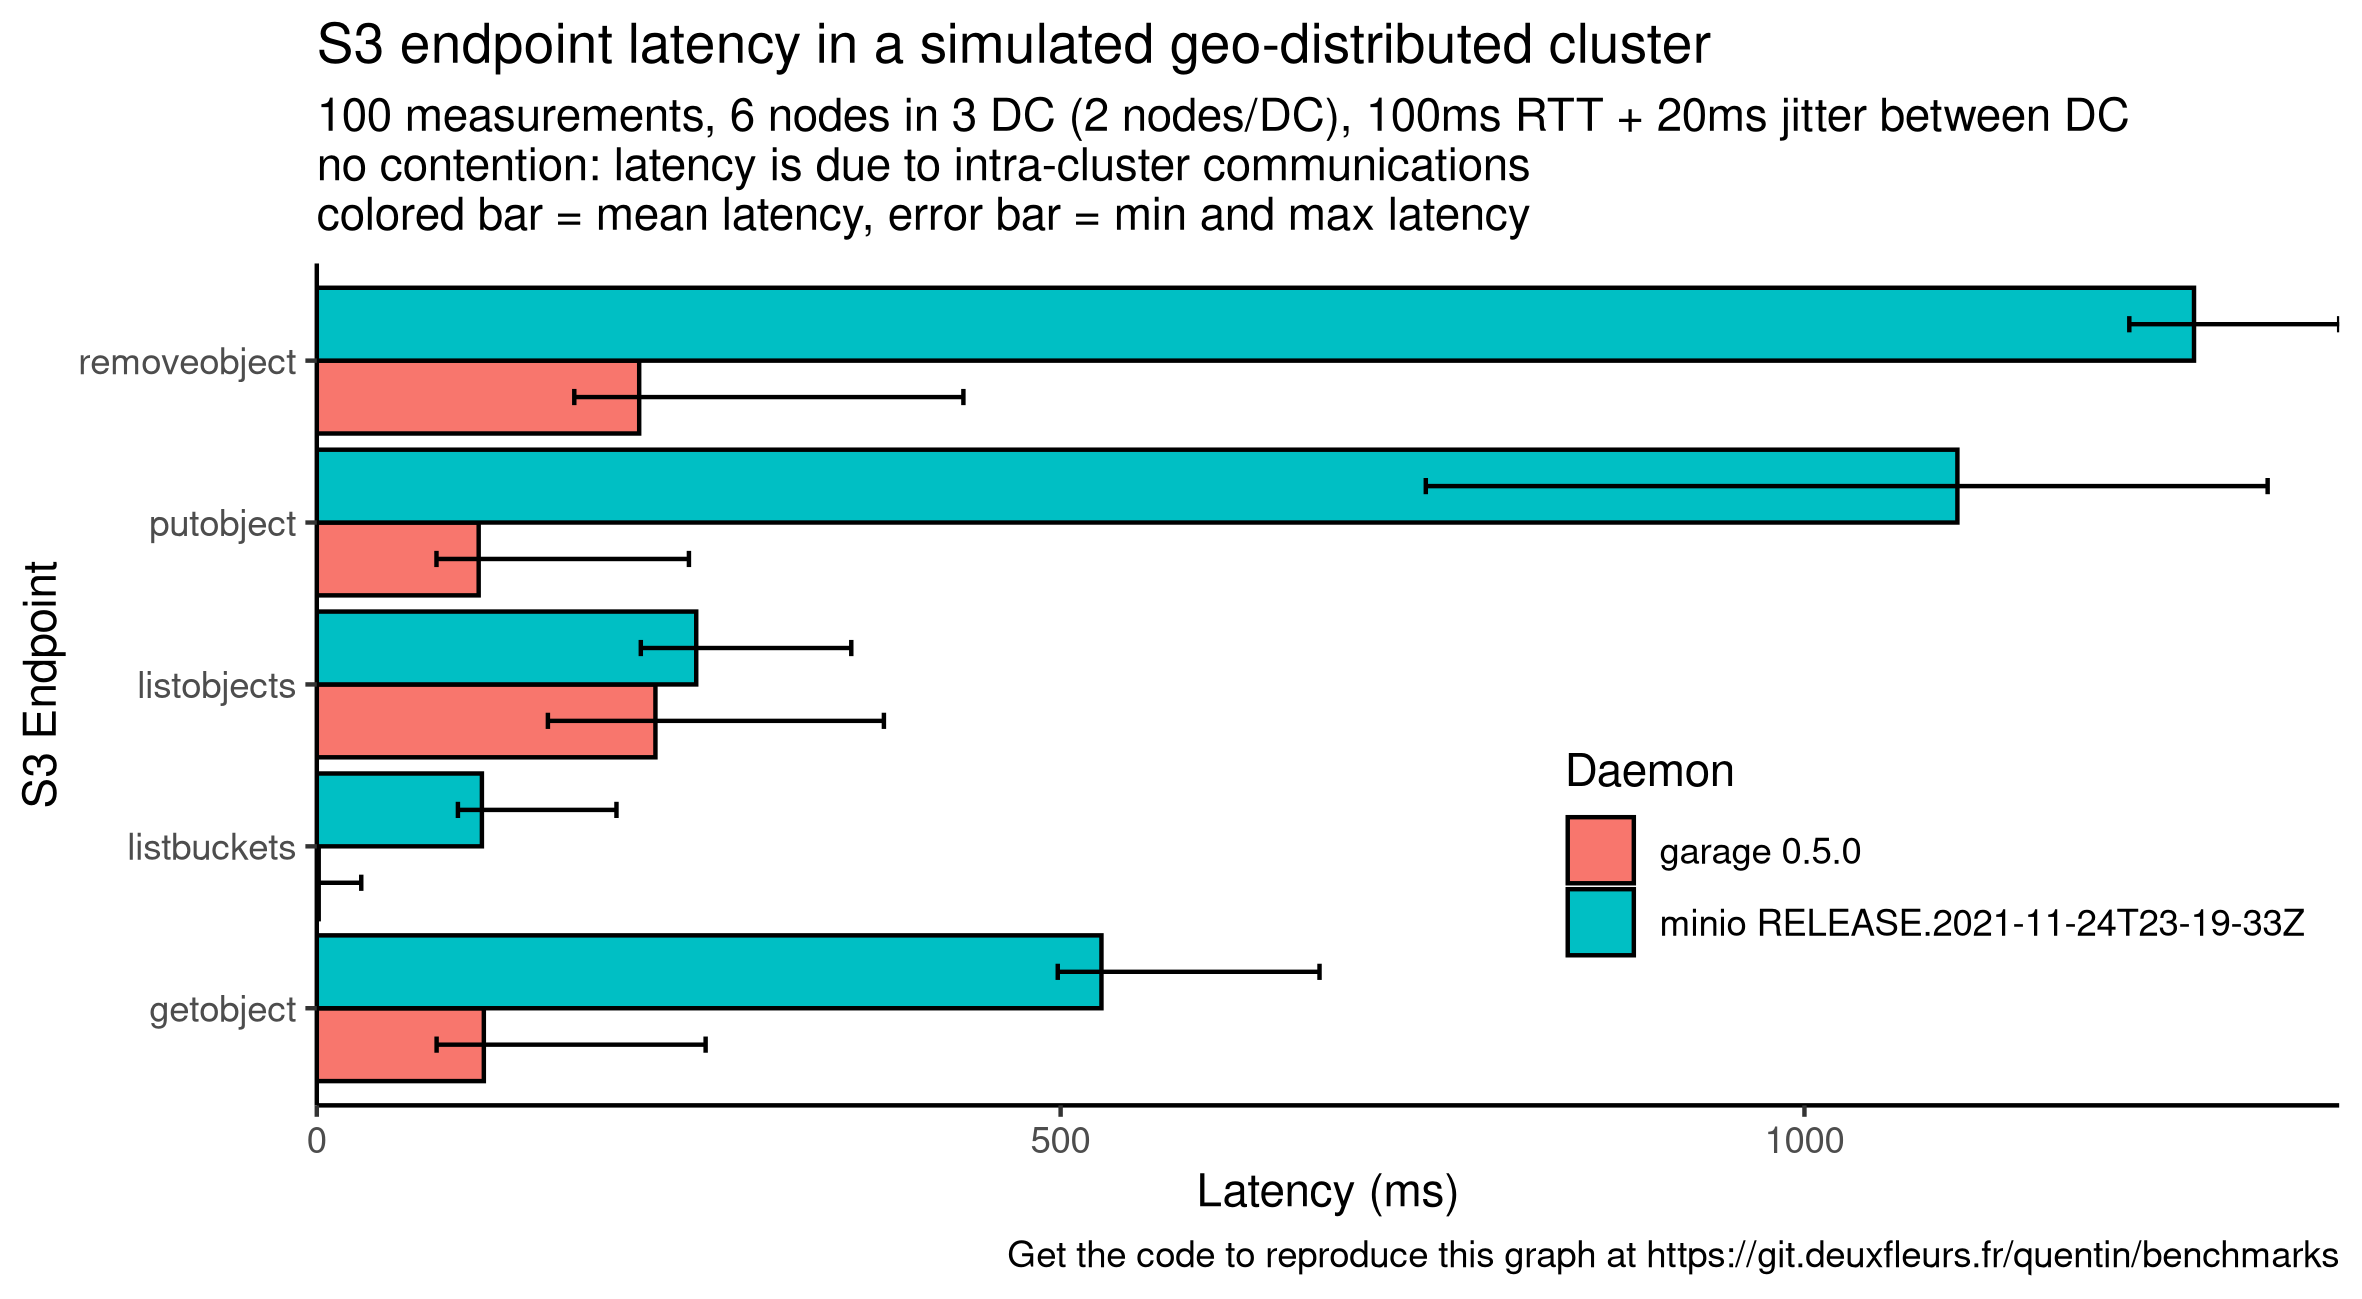
\includegraphics[width=.8\linewidth]{assets/endpoint-latency-dc.png}
	\end{center}
\end{frame}

\begin{frame}
	\frametitle{What can we implement without consensus?}
	\begin{itemize}
		\item Any \textbf{conflict-free replicated data type} (CRDT)
			\vspace{1em}
		\item Non-transactional key-value stores such as S3 are equivalent to a simple CRDT:\\
			a \textbf{last-writer-wins registry}
			\vspace{1em}
		\item \textbf{Read-after-write consistency} can be implemented
			using quorums on read and write operations
			\vspace{1em}
		\item \textbf{Monotonicity of reads} can be implemented with repair-on-read\\
			(makes reads more costly, not implemented in Garage)
	\end{itemize}
\end{frame}

\begin{frame}
	\frametitle{CRDTs and quorums: read-after-write consistency}
	\begin{figure}
		\centering
		\def\svgwidth{.8\textwidth}
		\only<1>{\import{assets/}{lattice1.pdf_tex}}%
		\only<2>{\import{assets/}{lattice2.pdf_tex}}%
		\only<3>{\import{assets/}{lattice3.pdf_tex}}%
		\only<4>{\import{assets/}{lattice4.pdf_tex}}%
		\only<5>{\import{assets/}{lattice5.pdf_tex}}%
		\only<6>{\import{assets/}{lattice6.pdf_tex}}%
		\only<7>{\import{assets/}{lattice7.pdf_tex}}%
		\only<8>{\import{assets/}{lattice8.pdf_tex}}%
	\end{figure}
\end{frame}

\begin{frame}
	\frametitle{CRDTs and quorums: read-after-write consistency}
	\textbf{Property:} If node $A$ did an operation $write(x)$ and received an OK response,\\
		\hspace{2cm} and node $B$ starts an operation $read()$ after $A$ received OK,\\
		\hspace{2cm} then $B$ will read a value $x' \sqsupseteq x$.

	\vspace{1em}

	\hspace{1em}
	\begin{minipage}{6.8cm}
		\textbf{Algorithm $write(x)$:}
		\begin{enumerate}
			\item Broadcast $write(x)$ to all nodes
			\item Wait for $k > n/2$ nodes to reply OK
			\item Return OK
		\end{enumerate}
	\end{minipage}
	\hfill
	\begin{minipage}{6.8cm}
		\vspace{1em}
		\textbf{Algorithm $read()$:}
		\begin{enumerate}
			\item Broadcast $read()$ to all nodes
			\item Wait for $k > n/2$ nodes to reply\\
				with values $x_1, \dots, x_k$
			\item Return $x_1 \sqcup \dots \sqcup x_k$
		\end{enumerate}
	\end{minipage}
	\hspace{1em}

	\vspace{2em}
	\textbf{Why does it work?} There is at least one node at the intersection between the two sets of nodes that replied to each request, that ``saw'' $x$ before the $read()$ started ($x_i \sqsupseteq x$).
\end{frame}

\begin{frame}
	\frametitle{CRDTs and quorums: monotonic-reads consistency}
	\begin{figure}
		\centering
		\def\svgwidth{.8\textwidth}
		\only<1>{\import{assets/}{latticeB_1.pdf_tex}}%
		\only<2>{\import{assets/}{latticeB_2.pdf_tex}}%
		\only<3>{\import{assets/}{latticeB_3.pdf_tex}}%
		\only<4>{\import{assets/}{latticeB_4.pdf_tex}}%
		\only<5>{\import{assets/}{latticeB_5.pdf_tex}}%
		\only<6>{\import{assets/}{latticeB_6.pdf_tex}}%
		\only<7>{\import{assets/}{latticeB_7.pdf_tex}}%
		\only<8>{\import{assets/}{latticeB_8.pdf_tex}}%
		\only<9>{\import{assets/}{latticeB_9.pdf_tex}}%
		\only<10>{\import{assets/}{latticeB_10.pdf_tex}}%
	\end{figure}
\end{frame}

\begin{frame}
	\frametitle{CRDTs and quorums: monotonic-reads consistency}
	\textbf{Property:} If node $A$ did an operation $read()$ and received $x$ as a response,\\
		\hspace{2cm} and node $B$ starts an operation $read()$ after $A$ received $x$,\\
		\hspace{2cm} then $B$ will read a value $x' \sqsupseteq x$.

	\vspace{1em}

	\textbf{Algorithm $read()$:}
	\begin{enumerate}
		\item Broadcast $read()$ to all nodes
		\item Wait for $k > n/2$ nodes to reply with values $x_1, \dots, x_k$
		\item If $x_i \ne x_j$ for some nodes $i$ and $j$,\\
			\hspace{1cm}then call $write(x_1 \sqcup \dots \sqcup x_k)$ and wait for OK from $k' > n/2$ nodes
		\item Return $x_1 \sqcup \dots \sqcup x_k$
	\end{enumerate}

	\vspace{1em}

	This makes reads slower in some cases, and is \textbf{not implemented in Garage}.
\end{frame}

\begin{frame}
	\frametitle{The hard parts we don't address (yet!)}
	\begin{itemize}
		\item Maintain consistency changes when nodes assigned to a partition change:\\
		\item TODO
	\end{itemize}
\end{frame}

\section{Going further than the S3 API}

\begin{frame}
	\frametitle{Further plans for Garage}
	\begin{center}
		\only<1>{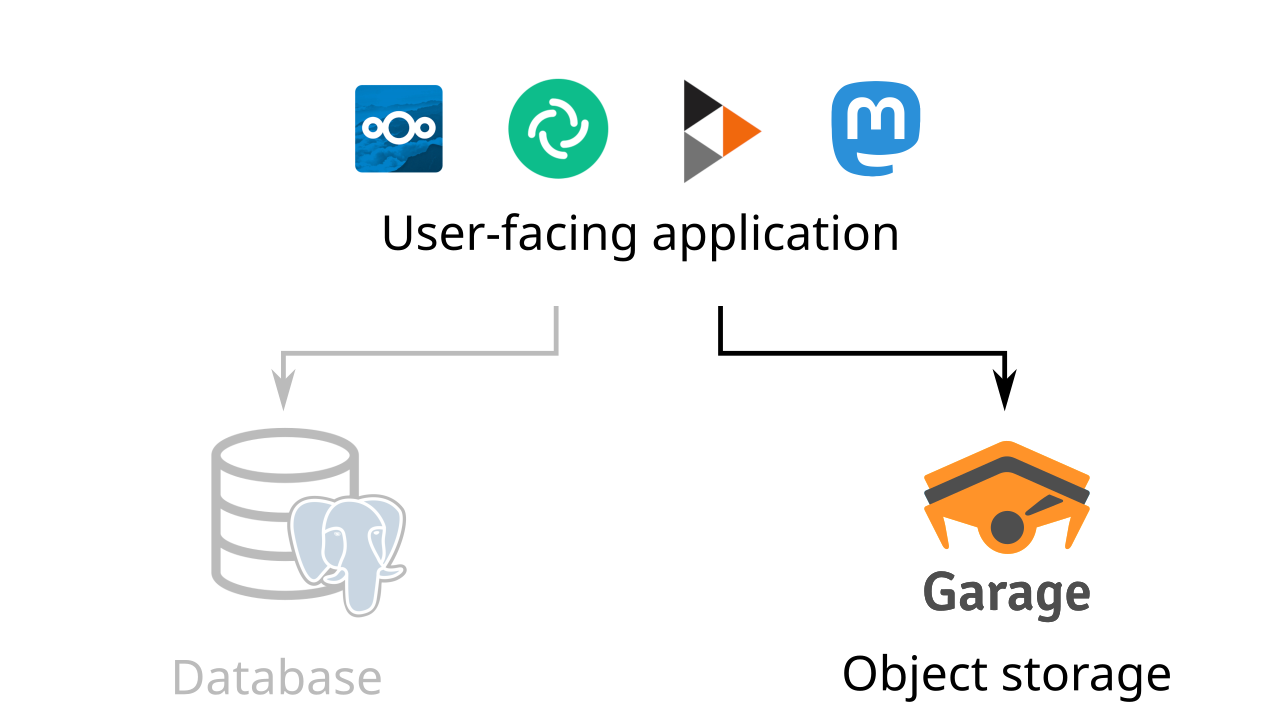
\includegraphics[width=.8\linewidth]{assets/slideB1.png}}%
		\only<2>{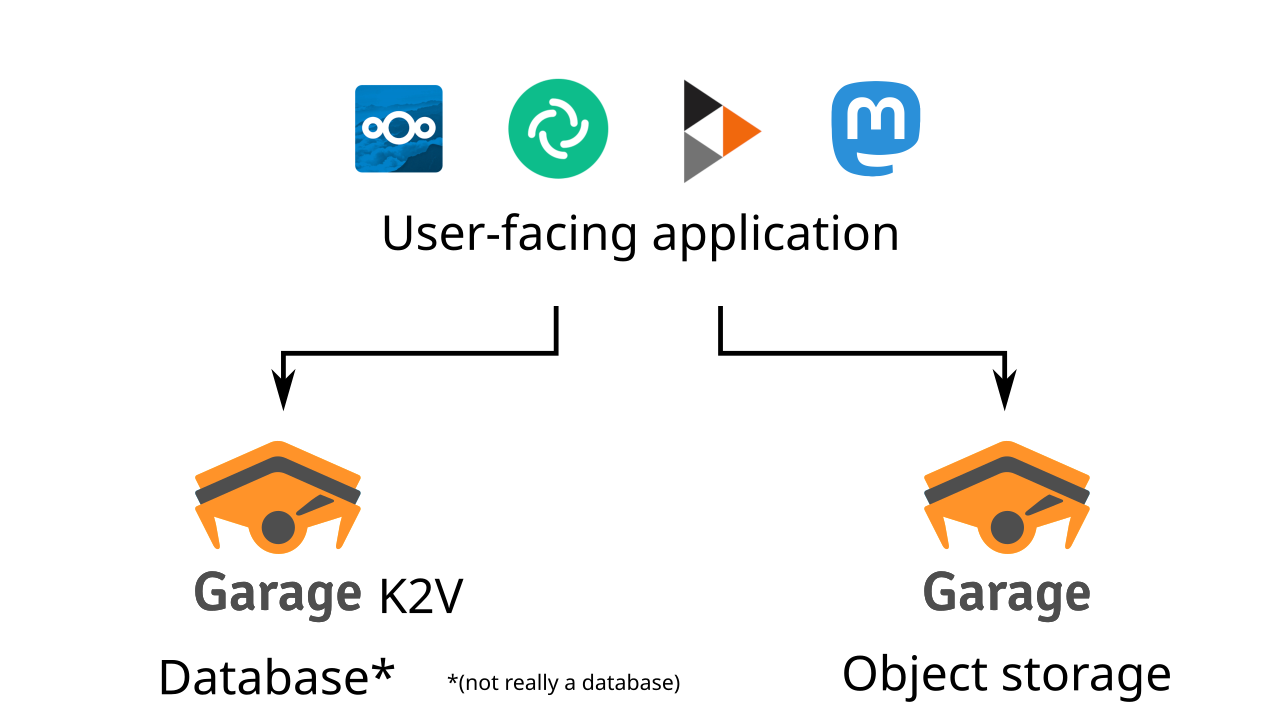
\includegraphics[width=.8\linewidth]{assets/slideB2.png}}%
		\only<3>{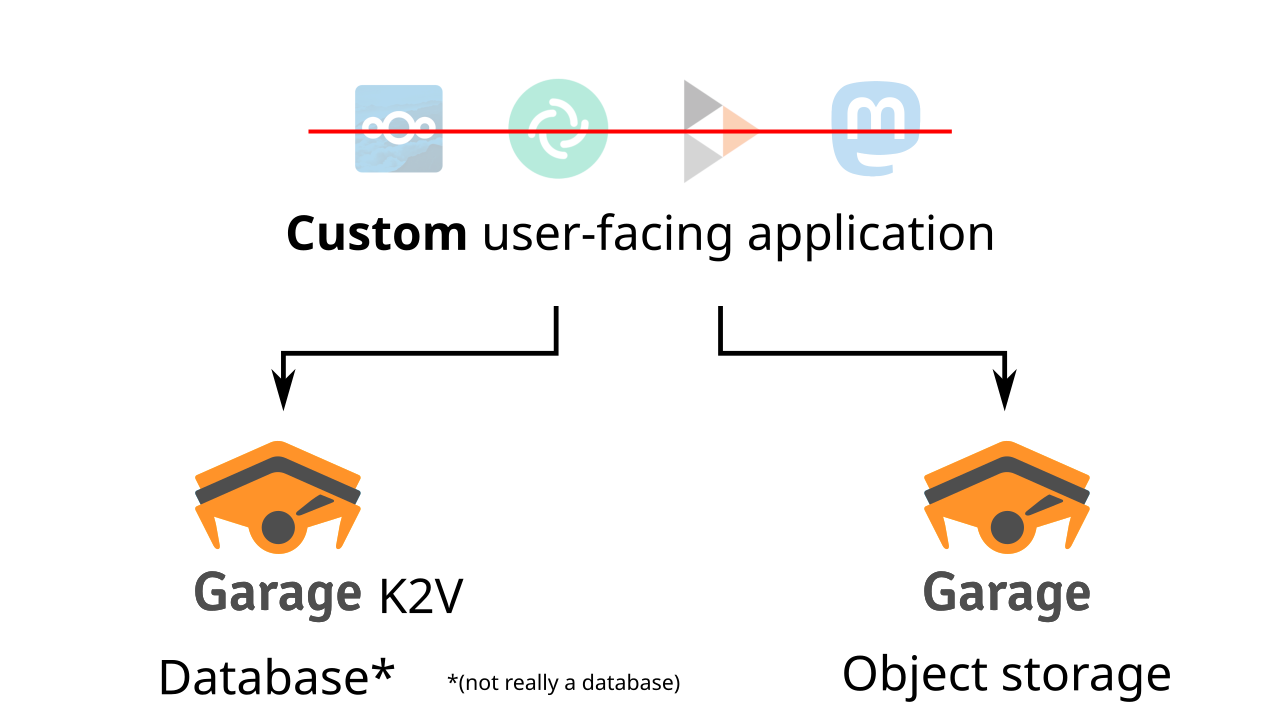
\includegraphics[width=.8\linewidth]{assets/slideB3.png}}%
	\end{center}
\end{frame}

\begin{frame}
	\frametitle{K2V Design}
	\begin{itemize}
		\item A new, custom, minimal API
			\vspace{1em}
		\item<2-> Exposes the partitoning mechanism of Garage\\
			K2V = partition key / sort key / value (like Dynamo)
			\vspace{1em}
		\item<3-> Coordination-free, CRDT-friendly (inspired by Riak)\\
			\vspace{1em}
		\item<4-> Cryptography-friendly: values are binary blobs
	\end{itemize}
\end{frame}

\begin{frame}
	\frametitle{Application: an e-mail storage server}
	\begin{center}
		\only<1>{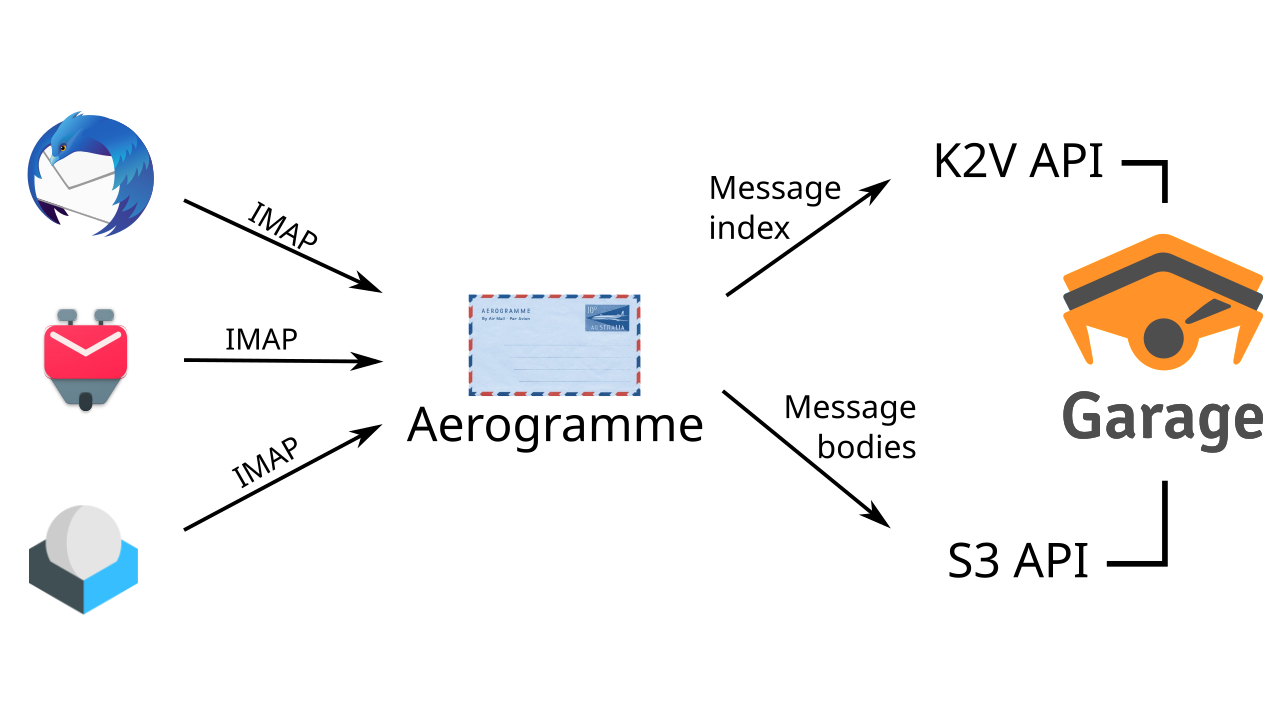
\includegraphics[width=.9\linewidth]{assets/aerogramme.png}}%
	\end{center}
\end{frame}

\begin{frame}
	\frametitle{A new model for building resilient software}
	\begin{itemize}
		\item Design a data model suited to K2V\\
			{\footnotesize (see Cassandra docs on porting SQL data models to Cassandra)}
			\vspace{1em}
			\begin{itemize}
				\item Use CRDTs or other eventually consistent data types (see e.g. Bayou)
					\vspace{1em}
				\item Store opaque binary blobs to provide End-to-End Encryption\\
			\end{itemize}
			\vspace{1em}
		\item Store big blobs (files) in S3
			\vspace{1em}
		\item Let Garage manage sharding, replication, failover, etc.
	\end{itemize}
\end{frame}

\begin{frame}
	\frametitle{Research perspectives}
	\begin{itemize}
		\item Write about Garage's global architecture \emph{(paper in progress)}
			\vspace{1em}
		\item Measure and improve Garage's performances
			\vspace{1em}
		\item Discuss the optimal layout algorithm, provide proofs
			\vspace{1em}
		\item Write about our proposed architecture for (E2EE) apps over K2V+S3
	\end{itemize}
\end{frame}

\begin{frame}
	\frametitle{Where to find us}
	\begin{center}
			\includegraphics[width=.25\linewidth]{../../logo/garage_hires.png}\\
			\vspace{-1em}
		\url{https://garagehq.deuxfleurs.fr/}\\
		\url{mailto:garagehq@deuxfleurs.fr}\\
		\texttt{\#garage:deuxfleurs.fr} on Matrix

		\vspace{1.5em}
			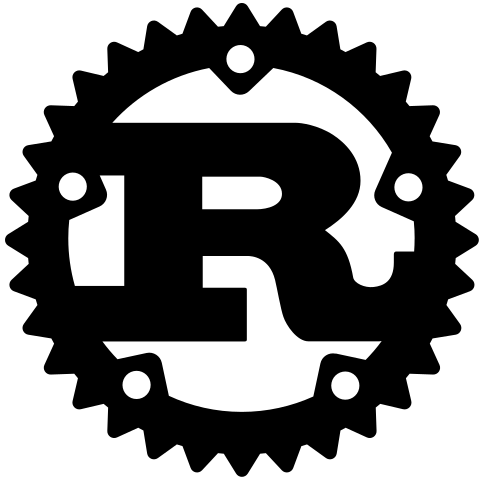
\includegraphics[width=.06\linewidth]{assets/rust_logo.png}
			
\includegraphics[width=.13\linewidth]{assets/AGPLv3_Logo.png}
	\end{center}
\end{frame}

\end{document}

%% vim: set ts=4 sw=4 tw=0 noet spelllang=en :
